\chapter{Container life cycle} \label{appendix:container-life-cycle}
During its life cycle, a container will go through five stages: creation, launch, execution, stopping and cleaning.  Those five steps are explained below and presented in figure \ref{fig:container-life-cycle}, along with the corresponding command for each presented tool.  Other optional stages (like pause/unpause) are not presented here.
\begin{enumerate}
\item\textbf{Create} This is the set-up phase, depending on the tool, the file system of the new container might be copied, or any other things that need to be done before launching the container.  This phase can only be done one time for each container.
\item\textbf{Launch} This is the proper instantiation of the container, the namespaces are created, the new file system is adopted.  Depending on the container, a complete init process might be executed.  This state can be repeated as many times as we want for a container, as long as it is in a stopped state.
\item\textbf{Execute} This corresponds to the execution of a process in the container.  This can be done as many times as we want for a container, as long as the container is running.
\item\textbf{Stop} This is when the container needs to be stopped, all running processes are killed, and the namespaces are exited.  No modification should be done on the filesystem, the storage of the container remains.
\item\textbf{Clean} This is the un-create phase, where we delete everything that was done during the creation phase.  The storage will be lost after this phase.
\end{enumerate}
\begin{figure}[!h]
  \begin{center}
    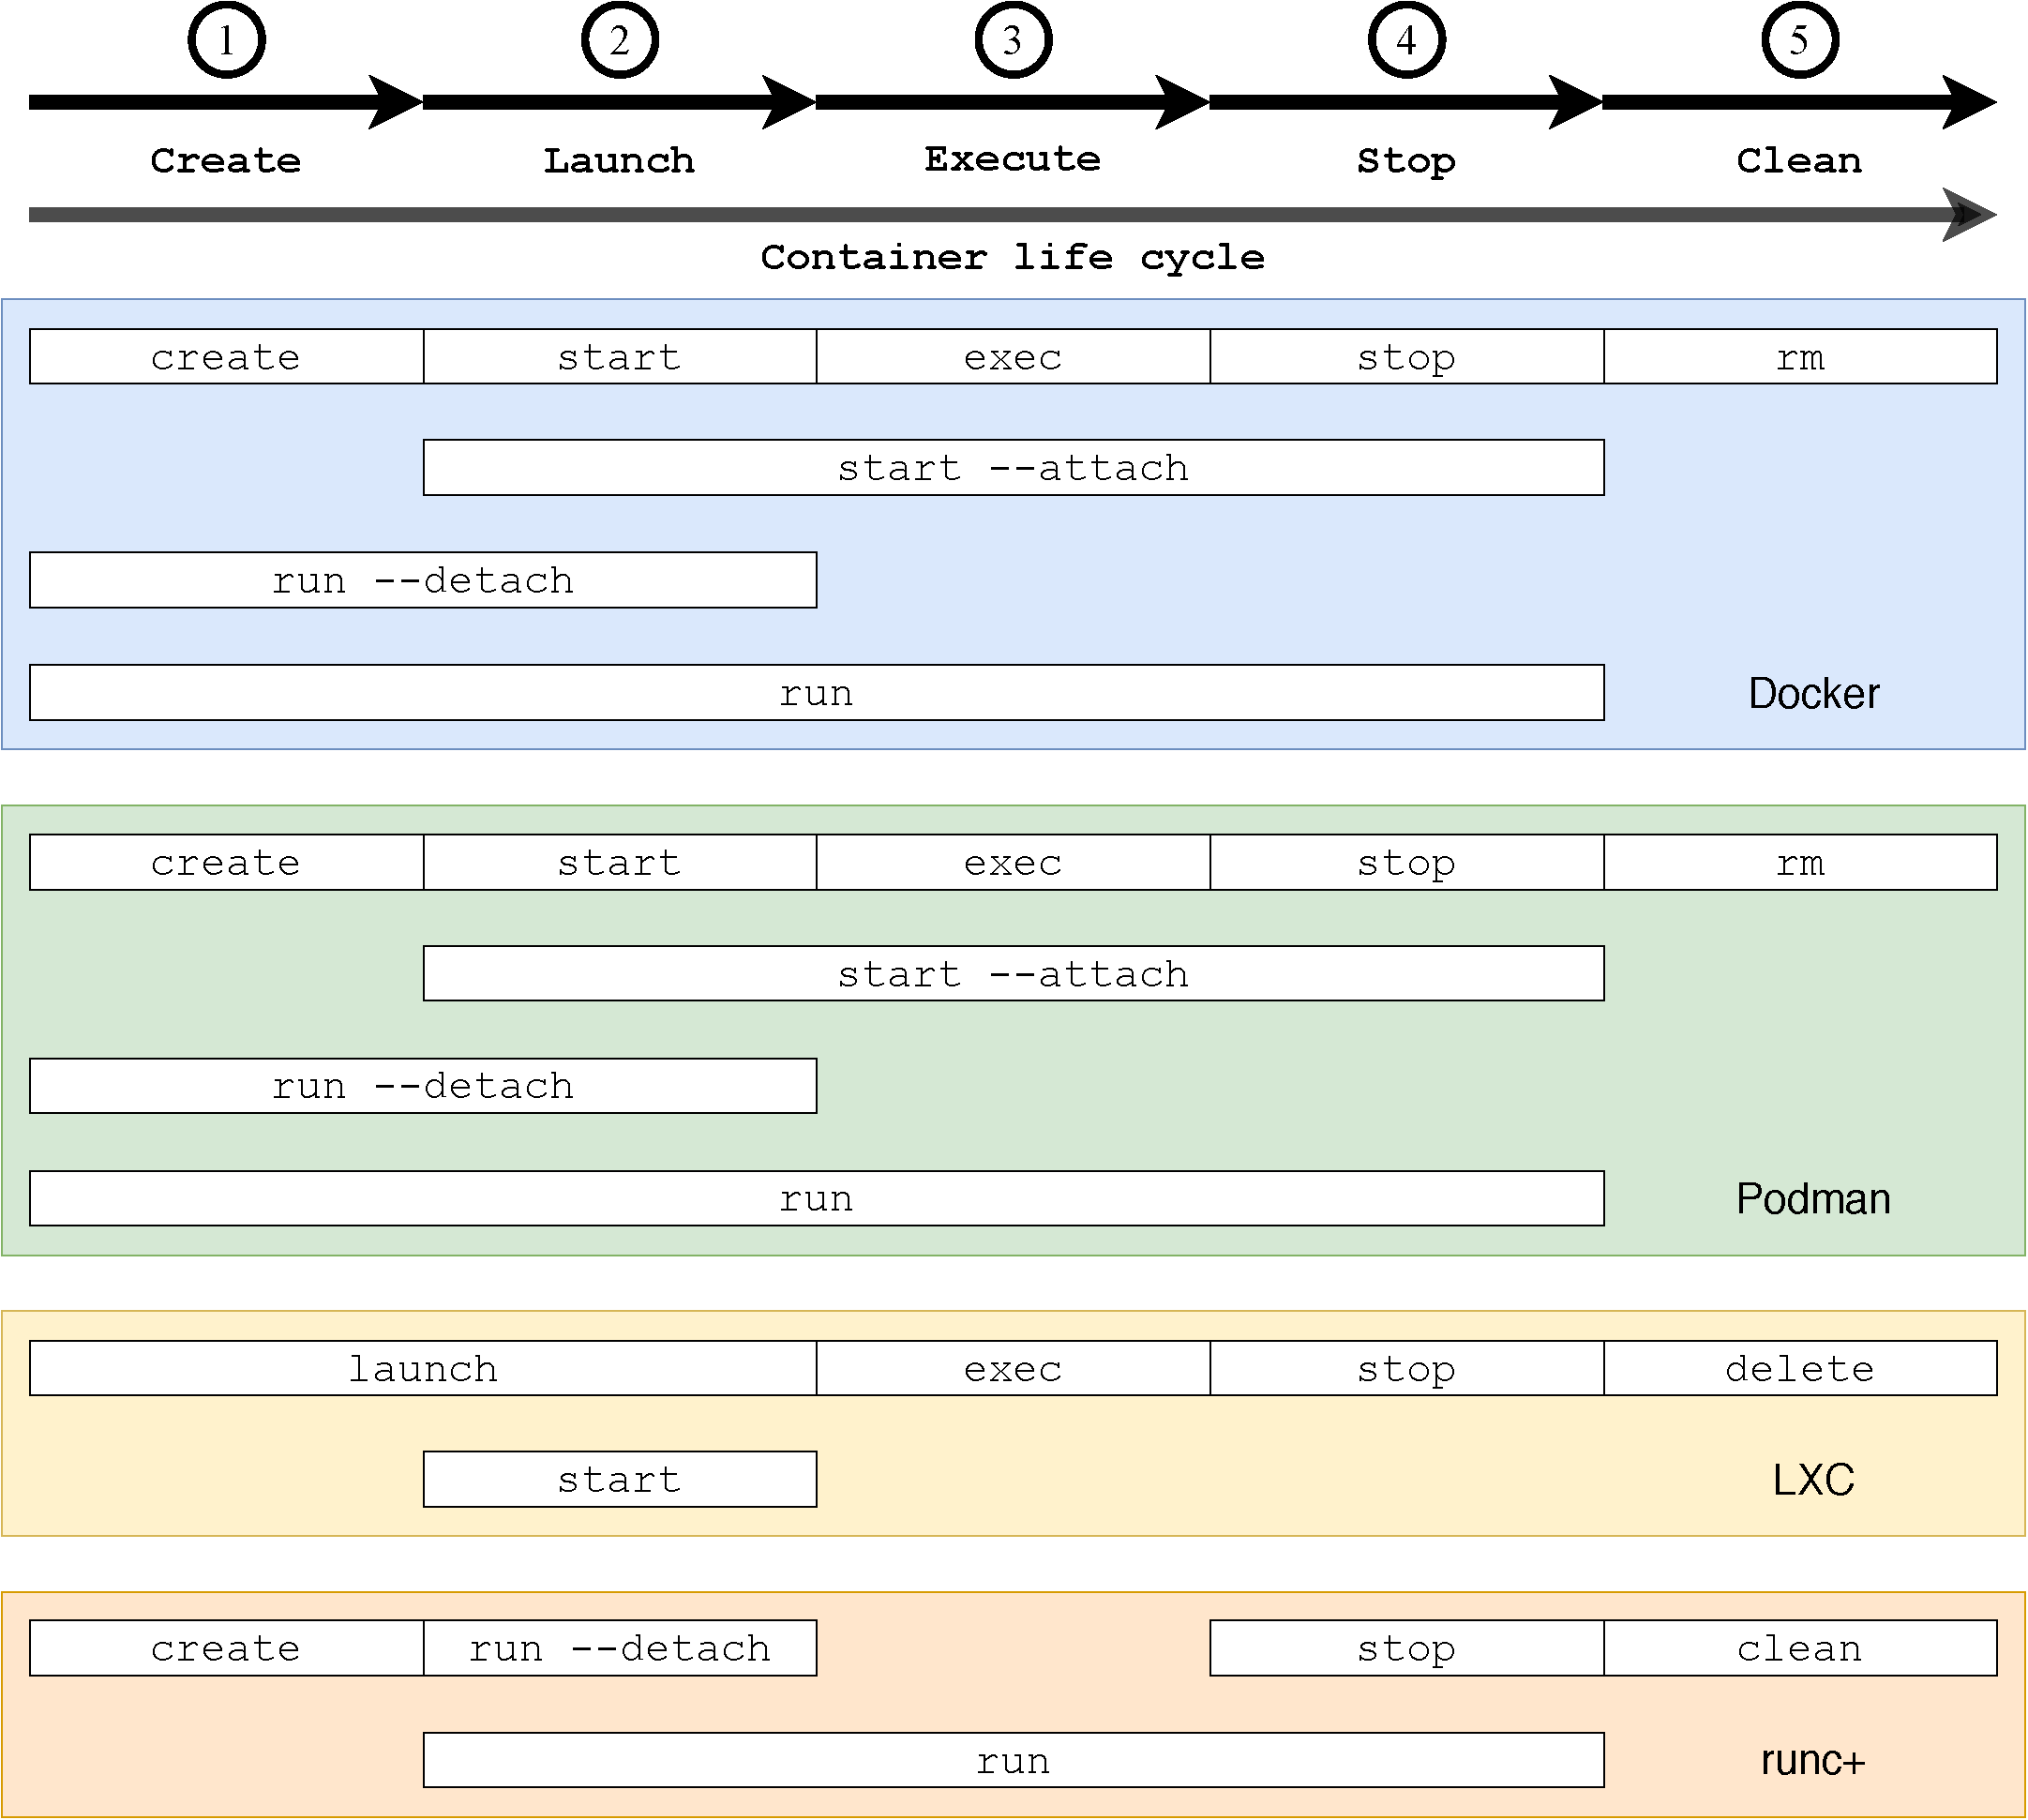
\includegraphics[width=\linewidth]{images/Container-life-cycle.pdf}
    \caption{Container life cycle and how to interact with it.}
    \label{fig:container-life-cycle}
  \end{center}
\end{figure}
